\let\negmedspace\undefined
\let\negthickspace\undefined
\documentclass[journal]{IEEEtran}
\usepackage[a5paper, margin=10mm, onecolumn]{geometry}
\usepackage{lmodern} 
\usepackage{tfrupee} 

\setlength{\headheight}{1cm} 
\setlength{\headsep}{0mm}     

\usepackage{gvv-book}
\usepackage{gvv}
\usepackage{cite}
\usepackage{amsmath,amssymb,amsfonts,amsthm}
\usepackage{algorithmic}
\usepackage{graphicx}
\usepackage{textcomp}
\usepackage{xcolor}
\usepackage{txfonts}
\usepackage{listings}
\usepackage{enumitem}
\usepackage{mathtools}
\usepackage{gensymb}
\usepackage{comment}
\usepackage[breaklinks=true]{hyperref}
\usepackage{tkz-euclide} 

\begin{document}

\bibliographystyle{IEEEtran}

\title{2.5.2}
\author{Revanth Siva Kumar D - EE25BTECH11048
}
{\let\newpage\relax\maketitle}

\textbf{Question} 
The points $(-4,0), (4,0), (0,3)$ are the vertices of a:
\begin{enumerate}[label=(\alph*)]
    \item right triangle
    \item isosceles triangle
    \item equilateral triangle
    \item scalene triangle
\end{enumerate}

\textbf{Solution:} 

\textbf{Step 1: Represent points as column vectors}


\begin{align}
\vec{A} = \myvec{-4\\0}, \quad 
\vec{B} = \myvec{4\\0}, \quad 
\vec{C} = \myvec{0\\3}
\end{align}

\textbf{Step 2: Check for right-angled triangle (perpendicular sides)}
\begin{align}
\vec{B}-\vec{A} &= \myvec{8\\0}, &
\vec{C}-\vec{A} &= \myvec{4\\3}, &
(\vec{B}-\vec{A})^\top (\vec{C}-\vec{A}) = \myvec{8&0}\myvec{4\\3} = 32 \neq 0 \\
\vec{A}-\vec{B} &= \myvec{-8\\0}, &
\vec{C}-\vec{B} &= \myvec{-4\\3}, &
(\vec{A}-\vec{B})^\top (\vec{C}-\vec{B}) = \myvec{-8&0}\myvec{-4\\3} = 32 \neq 0 \\
\vec{A}-\vec{C} &= \myvec{-4\\-3}, &
\vec{B}-\vec{C} &= \myvec{4\\-3}, &
(\vec{A}-\vec{C})^\top (\vec{B}-\vec{C}) = \myvec{-4&-3}\myvec{4\\-3} = -7 \neq 0
\end{align}
Since no pair of sides is perpendicular, the triangle is not right-angled.\\
\textbf{Step 3: Check for isosceles triangle (perpendicular bisector method)}
\begin{align}
\text{Midpoint of } AB: \quad \vec{M} = \frac{\vec{A}+\vec{B}}{2} = \myvec{0\\0} \\
\vec{C}-\vec{M} = \myvec{0\\3}-\myvec{0\\0} = \myvec{0\\3} \\
\vec{B}-\vec{A} = \myvec{8\\0} \\
(\vec{B}-\vec{A})^\top (\vec{C}-\vec{M}) = \myvec{8&0}\myvec{0\\3} = 0
\end{align}


\begin{align*}
\text{Hence, } C \text{ lies on the perpendicular bisector of } AB.\\
AC = BC = 5 \implies \triangle ABC \text{ is isosceles.}
\end{align*}


\textbf{Conclusion:} Therefore, the triangle with vertices $(-4,0), (4,0), (0,3)$ is an \textbf{isosceles triangle} with $AC = BC = 5$.

\begin{figure}[H]
    \centering
    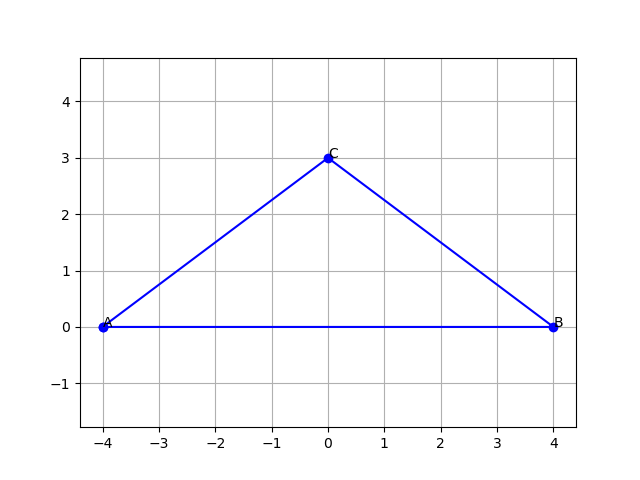
\includegraphics[width=0.8\columnwidth]{figs/Figure_1.png}
    \caption{Shared Output Plot}
    \label{fig:fig1}
\end{figure}

\begin{figure}[H]
    \centering
    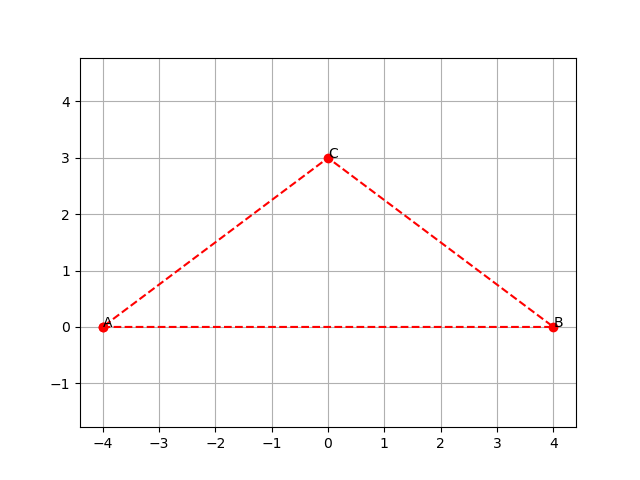
\includegraphics[width=0.8\columnwidth]{figs/Figure_2.png}
    \caption{Direct Python code plot}
    \label{fig:fig2}
\end{figure}
\end{document}

